%&pdflatex
\documentclass[12pt]{okstate-thesis}
\usepackage{graphicx}
%\usepackage[draft]{graphicx}
%\usepackage{subfigure}
%\usepackage{verbatim}
%\usepackage{enumerate}
%\usepackage{amsmath}
%\usepackage{amscd}
%\usepackage{array}
%\usepackage{color}
%\usepackage{amsxtra}
%\usepackage{amstext}
%\usepackage{amssymb}
%\usepackage{hyperref}
%\usepackage{mathrsfs}
%\usepackage{latexsym}
%\usepackage{newlfont}
%\usepackage{indentfirst,color}
%\usepackage{doublespace}
%
\suppressfloats %\nofiles


\usepackage[parfill]{parskip}    		% Activate to begin paragraphs with an empty line rather than an %indent
\usepackage{graphicx}				% Use pdf, png, jpg, or eps§ with pdflatex; use eps in DVI mode
\graphicspath{{New_Images/}}
								% TeX will automatically convert eps --> pdf in pdflatex		
\usepackage{amssymb}
\usepackage{cite}
\usepackage{textcomp}
\usepackage{csquotes}
\usepackage{algpseudocode}
\usepackage{algorithm}
\usepackage{fixltx2e}
\usepackage{hyperref}
\usepackage{setspace}



\title{A Centralized Energy-Efficient Model for Increasing the Information Gathered in Wireless Sensor Networks}

\author{Sushyanth Pamulaparthy}

\degreeone{Bachelor of Technology in Information Technology \\
        Jawaharlal Nehru Technological University \\
        Hyderabad, Telangana, India \\
        2013}
        
%\degreetwo{Bachelor of Nothing in Foo\\
%        Prestigious University\\
%        My head, Universe\\
%        2012}
\degreesought{Master of Science}
\degreedate{July, 2015}
\majorfield{Computer Science}
\adviser{Dr. Christopher Crick}
\chairOne{Dr. Eric Chan-Tin}
\chairTwo{Dr. Johnson Thomas}
%\chairThree{name 3}
%\chairFour{name}
% If you've got more you're screwed anyway, but you can read the class file
% to figure it out.
%
\begin{document}
\frontmatter
\maketitle
\makeapproval{3} % Number denotes total number of required signatures (max 5)


\begin{acknowledge}
    `Life may be tough, but I've got a God that's tougher'. Firstly, I would like to thank God for all his blessings, helping me complete my thesis. I would like to express my sincerest gratitude towards my adviser, Dr. Christopher Crick, who has supported me throughout my thesis with his creative ideas and invaluable suggestions. I could not have asked for a better adviser and certainly would not have completed the thesis without his time, support and guidance.

I would like to take this opportunity to also thank my parents, brother, sister-in-law and sisters for the suggestions, support and attention they have provided me throughout my life. Last but not the least, I thank my friends for their unwavering support.
    \\[10\baselineskip]
\end{acknowledge}
\begin{abstract} % Creates abstract
    A Wireless Sensor Network (WSN) consists of numerous sensor nodes
spread over a wide area to gather information and transmit it to a
sink node, which then sends it to the end user for analysis. Such
networks have a wide range of applications in areas like health,
military, security, wildlife monitoring, etc. These sensors gather
huge amounts of data, not all of which is important to the end
user. Only a few sensors at any given point of time have valuable
information.  Identifying such sensors consistently can help us
increase the Value of Information (VoI) of a system. We know that
sensors generally have limited resources in terms of memory capacity,
power supply and communication bandwidth. Hence, it is important to
take energy-efficiency into consideration while implementing an
approach.

In order to address the above problems, we propose a centralized
network model which makes use of Information Entropy to determine the
theoretical upper bound on the VoI available in a network. We also
provide a probabilistic sensor selection algorithm to consistently
select the most informative sensor, enabling the model to increase the
amount of information gathered from a network. Simulation results show
that our approach gathers more information, especially at low ping
rates, when compared with several state-of-the-art models. To our
knowledge, this is the first implementation of a VoI-based approach
for a centralized WSN that is intended to efficiently maximize the
amount of information gathered from the system.
\end{abstract}
\tableofcontents
%\listoftables
\listoffigures
%\msp    %========  single space text.
        %========  For the final version, this command should not be used.

%\makeapproval{5}\addtocounter{placeholder}{-1}    %% Comment this in the final copy. This is for electronic copy
%\begin{nomenclature}
%	\input{notation}
%\end{nomenclature}

%====================== main  body of the dissertation ==========================
\mainmatter
\chapter{INTRODUCTION}
A Wireless Sensor Network is a collection of a huge number of sensor
nodes that are spread over a wide area and are responsible for
sensing, storing and transmitting information. A typical sensor node
consists of a radio, responsible for transmitting and receiving
information; a battery, which is the main energy source; a
micro-controller, which is a small computer on a chip, responsible for
performing computation and processing; an analog circuit and a sensor
interface.

Research on WSNs has been quite prevalent over the past decade as they
can be easily deployed in harsh environmental conditions, they are
cheap and are easy to maintain. More recently, advancements in
wireless technologies and wireless communication has led to widespread
use of sensors in applications like health, military, security,
agriculture, and wildlife monitoring. With such advancements, research
has also spread into several domains and has led to the development of
several architectures for sensor arrangement
\cite{akyildiz2002wireless}; made deployment of sensors easier; made
them cheaper and made them more scalable than ever. WSN sensor
architectures are commonly implemented in either centralized or
distributed fashion.  In a centralized network, the sink node (which
is usually considered to have unlimited resources in terms of
processing and energy) has complete control of the network and is
responsible for sensor deployment and resource allocation. This means
there is less burden on the sensor nodes and no self-organization
costs are inposed on them. On the other hand, in a distributed
network, sensors govern themselves and are responsible for deployment,
allocation of resources and communication with neighboring sensors to
transmit information to the sink node.

Let us consider an example scenario where a number of cheap, dumb
sensors are spread over an agricultural field in a distributed manner
to monitor agricultural factors like amount of water required for
cultivation, amount of fertilizer required, depth at which a seed must
be sown, etc. A decentralized arrangement for this network has the
following flaws: first, each sensor communicates with its neighboring
sensor(s) to transmit its information and, at the same time, it is
involved in passing information of other sensors' data
\cite{akyildiz2002wireless}. This means that the number of
communications being performed by each sensor in such a setting is
potentially greater than the network's energy budget can afford, as we
know that data transmission consumes more energy than any other sensor
network activity \cite{torres2006energy}. Hence, such an approach will
deplete the sensors' energy in short order, and the expensive process
of retrieval and redeployment must take place. Second, certain sensors
located close to the sink get exhausted quicker in comparison to other
sensors, as most sensors' data needs to pass through one of these
sensors \cite{heinzelman2002application}. Hence, for scenarios like
the one mentioned above and many others like monitoring of buildings,
it is often advisable to opt for a centralized architecture like the
one depicted in Figure \ref{cwsn}, which eliminates the flaws
mentioned above.

\begin{figure}
\begin{center}
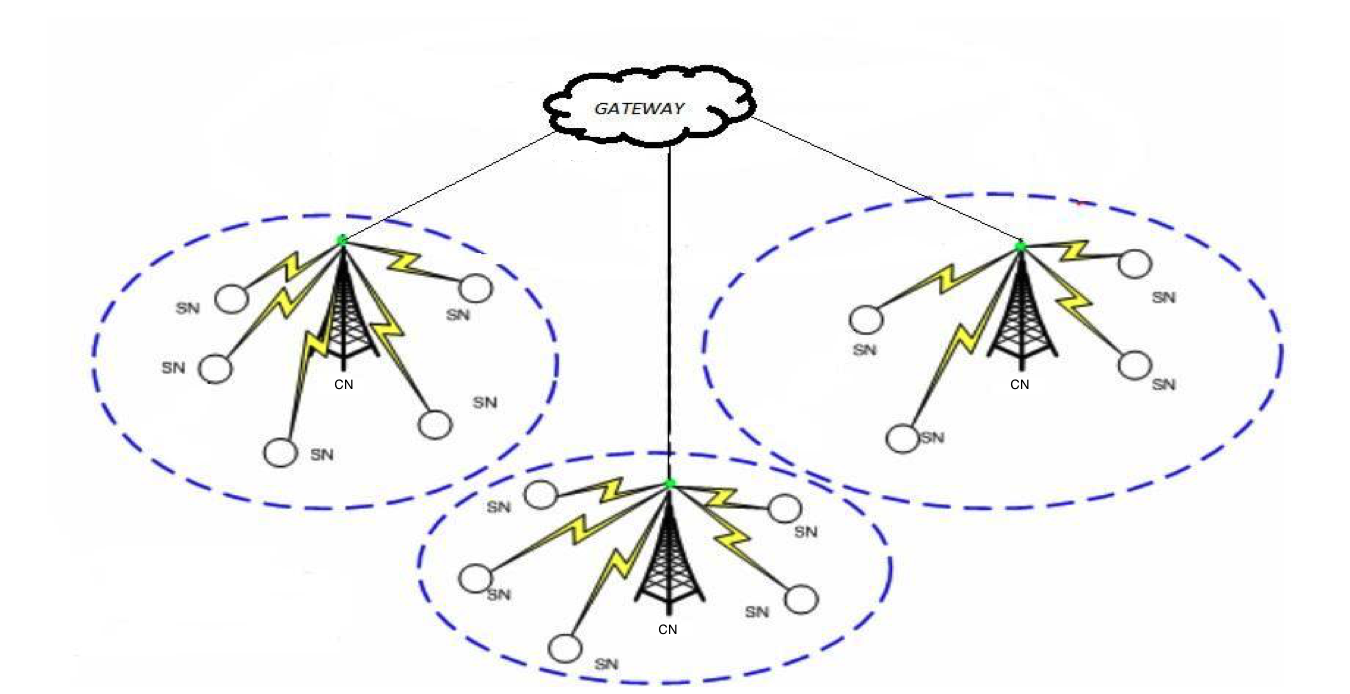
\includegraphics[height = 80mm, width = 150mm, scale = 2]{figs/CWSN}
\caption{A centralized WSN solution to WSNs on an energy budget}
\label{cwsn}
\end{center}
\end{figure}

However, in order to take advantage of the benefits mentioned above,
we will have to deal with several problems associated with
WSNs. Probably the most important of such problems is to improve the
energy-efficiency of the sensors within the WSN. This is because the
sensors ordinarily have small, low-capacity batteries as their only
energy source. Once a battery is drained it can be very expensive to
replace it, and more importantly, we will lose the ability of the
network to give us an accurate measure of the sensing environment
during the period when the sensor is offline. Hence, it is crucial
that we prolong the lifetime of sensors by improving the energy
efficiency of a sensor network deployment scheme. Over the years,
several approaches have been proposed to address this problem.

Another problem lies in the fact that not all the sensors at every
moment of time provide the best information. Most of the time, sensors
send redundant information, which is non-informative in terms of
entropy. Many approaches like data fusion, data aggregation,
clustering etc. have been proposed to reduce redundant data
\cite{abbasi2007survey} \cite{rajagopalan2006data}. Also, several
approaches have been proposed in order to maximize the amount of
information gathered from a system \cite{ji2014data}. This problem has
also been proven as NP-Hard \cite{chou2009energy}.

In this paper, we propose an approach that makes use of Information
Entropy to determine the theoretical upper bound on the VoI available
in a network and to increase the amount of information gathered from
the network. We achieve this by identifying the most informative
sensors consistently and query/ping them more often on comparison to
others, thereby increasing the overall information gathered from the
system.

In order to show energy-efficiency, our approach varies the rate of
sampling to prove that it gathers more information from the sensors
even at low sampling rates, instead of transmitting information to the
central node whenever a change is seen -- which eventually leads to
making excessive, unnecessary transmissions and depleting the sensors'
energy more quickly. The simulation results shown below are concrete
proof that our approach (in comparison with two state-of-the-art
models) gathers more information at every ping rate taken into
consideration. These results are further evidence for the fact that
our model gathers more information per ping and is energy-efficient in
comparison.
\label{intro}
\chapter{REVIEW OF LITERATURE}
The main goal of a WSN is to collect data from the sensing environment
and send it to the end user for analysis. Research to maximize this
information being collected has led to development of several models
\cite{abuarqoub2012overview}. Generally, in order to increase the
overall information to be gathered, the sensors will have to sense
more and transmit that sensed information to the sink. We know that
energy conservation of sensor nodes is vital in WSNs and we cannot
afford the communication costs to be high, as it will lead to
depletion of the network sooner than expected. There have only been a
handful of papers published considering both these issues together.
Our approach is the first to implement a VoI-based technique in
centralized networks, in order to address increasing the information
gathered while simultaneously reducing overall communications. Before
we take a look at our technical approach, we will look at some of the
recent work done in these areas.

Various techniques are employed among multi-hop communication
approaches, such as sensor shutdowns and censoring, are usually used
to increase the energy-efficiency in WSNs. We should keep in mind that
energy management in WSNs involves not only reducing the energy
consumption of a single sensor node but also maximizing the lifetime
of the entire network.

Data aggregation is one approach, which considers the problem of
sending redundant information to the sink and aims to reduce such
information reaching the sink. Several data aggregation techniques can
be seen in \cite{rajagopalan2006data}, where authors show how
redundant data proves to be expensive in terms of system performance,
energy consumption and congestion. However, authors in
\cite{galluccio2008efficient} have proven that aggregation implies
performing more complex operations than simply relaying traffic, and
this can lead to an increase, rather than a decrease, in the overall
energy consumption. Also, higher aggregation could be costly in terms
of loss of information.

In \cite{sinha2013performance}, authors propose a distributed
entropy-based data aggregation model with the aim of sending only
surprising information to the sink node. This is one work closely
related to our approach as authors use propose local and global
probability models for computing entropy. We, on the other hand,
calculate entropy of the data and use a probability approach to
increase the amount of information gathered from the system by
reducing the overall transmissions. In \cite{sinha2013performance},
authors use the entropy computed in data aggregation and from
\cite{galluccio2008efficient}, we know that aggregation is not easy to
handle. In contrast, we use the entropy calculated to consistently
select the most informative sensor at every instant thereby increasing
the overall information gathered.

In \cite{chou2009energy}, authors propose an adaptive algorithm based
on ``Adaptive Compressive Sensing" to obtain an accurate
approximation of the sensing field with minimum energy consumption as
possible. Here, the sink node makes projections to the sensor nodes if
the readings transmitted by them are not satisfactory. Authors jointly
optimize the routing and compression to obtain optimal measurement,
which greatly increases the complexity.  On the other hand, our VoI
based approach uses entropy to firstly, determine the theoretical
maximum amount of information available and secondly, to randomly identify
the informative sensors based on their weighted VoI. From the results shown
below, we show that our model is on course to reach the theoretical maximum
computed which means we will have a very accurate measure of the environment
being sensed depending on the number of transmissions.

Clustering is another approach where several techniques have been
proposed, particularly to increase the energy-efficiency. The main
goal is to reduce the number of transmissions by sending information
collected by each sensor of a cluster to a particular sensor, called a
cluster head (CH). CHs are usually responsible for processing,
filtering, aggregating and transmitting non-redundant information to
the sink node \cite{heinzelman2000energy} \cite{lindsey2002pegasis}
\cite{younis2004heed}. Authors in \cite{muruganathan2005centralized}
propose a clustering approach in a centralized WSN to increase the
energy-efficiency. Here, CHs are chosen based on the amount of energy
available to the sensors. This means that every sensor within the
network has to have on-board processing abilities, which may impose
higher costs on the network's energy budget than it can afford.
Moreover, allocation of additional resources to the elected CH is a
problem, as it should have the abilities to perform additional tasks
and transmit information to the sink node.

On the other hand, our approach assumes the CN to be responsible for
performing the computations, leaving the sensor nodes to gather
information and send it to the CN upon request. We increase the amount
of information gathered from the system by calculating the entropy of
the data and using it to randomly query the sensors based on the current
weighted VoI. Moreover, our approach does not consider any inter-cluster
communications to be involved thereby further reducing the transmissions
and hence saving energy. We compare the implementation of our model to
the model proposed in \cite{muruganathan2005centralized}, where performance
improvement can be clearly observed.
	
%WORK ON EQUATION
%\begin{equation}
%\(Energy consumption (for \cite{maleki2011energy}) = Energy for (Gathering + Computation + Start-Up + Transmission)\)
%\end{equation}
Recently, self-censoring has become a major focus of research. This is
a distributed, in-network processing technique where sensors function
independently and are responsible for performing computations to
determine whether to send data to the sink node or not
\cite{rago1996censoring} \cite{jiang2005fusion}
\cite{axell2012spectrum}.  In this scheme, sensors only send
measurements that are deemed sufficiently informative, thereby
reducing the number of transmissions being made by the sensors. In
\cite{maleki2011energy}, authors implement a sleep/wake mechanism in
the state-of-the-art self-censoring technique to enhance the energy
efficiency. Here, a sleeping and censoring combined scheme is proposed
to jointly optimize the energy consumption cost under the optimal
sleeping constraint and the censoring thresholds. However, authors in
\cite{cho2001energy} have proved that sensor start-up can consume more
energy than information transmission. Using this demonstration, we can
say that each sensor consumes energy for gathering information,
performing computation, sensor start-up or wake-up and for
transmitting information, hence depleting the node faster than normal.
	
Our approach, in comparison, considers a model wherein sensors consume
energy only for sensing and transmitting information to the sink
node. Our approach considers the information content of every sensor's
readings, calculates the entropy for the information, and uses a
probabilistic approach to select the most informative sensor
consistently.

In \cite{rago1996censoring}, a censoring approach is used to reduce
the number of transmissions to the sink.  They propose a model based
on the likelihood ratio (LR). Sensors only transmit information to the
sink node if the information gathered by the sensor exceeds the LR
determined. LR is calculated using the following equation
\begin{equation}
LR = (Sensitivity) / (1-Specificity) %NUMBER!!!!            (1)
\end{equation}
This can be explained as the dual of the ratio of the probability of
false positives and false negatives.

Our model, on the other hand, uses a VoI-based technique using entropy
to determine information in the system. This entropy determines the
sensor to be selected for querying, and our model increases the
information gathered using fewer communications (or ``pings''),
therefore improving the energy-efficiency. Simulation results show how
our approach outperforms this model by gathering more amount of
information per ping.
\chapter{METHODOLOGY}
As we have seen in the previous section, research incorporating both
information extraction and energy-efficiency in WSNs is limited,
particularly in centralized networks. In this paper, we consider a WSN
organized in a centralized fashion, where all the sensor nodes are
deployed over a wide area. There can be multiple central nodes
(denoted by CN) depending on the area and number of sensor nodes being
deployed. However, we will be considering only one CN for the networks
we are dealing with in this paper. In this paper, we assume that all
sensors have the same sensing range and consume the same energy for
performing activities like data transmission and reception. Also, we
assume that the identity and position of each sensor are fixed and
known both to the CN and the sensor itself. Additionally, we consider
the CN to have unlimited resources in terms of energy and processing
abilities. Finally, we assume that energy consumption for sensing is
negligible, which is a reasonable consideration
\cite{hu2006deploying}.

In this paper, we will compute the amount of information extracted by
examining the total number of transmissions required to collect this
information from the sensing field. This work distinguishes itself
from existing works \cite{chou2009energy} in that it uses a
probability-based sensor selection scheme to increase the information
gathered and to improve the energy-efficiency of the entire network.

\section{Theoretical Maximum VoI (TM\textsubscript {VoI})}
In order to evaluate the information that our approach is extracting
from the network, it is important to compute a theoretical maximum for
the amount of information present within the system.  Doing so also
provides an idea of the accuracy of a given model's sensing field. We
obtain the TM\textsubscript {VoI} using an entropy-based approach, as
shown in Algorithm \ref{tmvoi}. To calculate the TM\textsubscript
{VoI}, we assume that the CN is able to query each of the sensor nodes
within the network \emph{whenever} the sensor detects new information.
We then sum the calculated entropies associated with those
values. Entropy provides the average amount of information present
within a message.  TM\textsubscript {VoI} is computed using the
following algorithm.

\begin{algorithm}
	\caption{Determining Theoretical Maximum VoI (TM\textsubscript {VoI})}
        \label{tmvoi}
	\textbf{Input:} Set of Sensors, SN \newline
	%TM\textsubscript {VoI}
	\textbf{Output:} Theoretical Maximum VoI, TM\textsubscript {VoI}
	 
	\begin{algorithmic}[1]
	\For {$i=0$ to $SN.length$}
	\State $data[i] = (SN[i])$\Comment{Initially, request data from each sensor in SN}
	\State $H (data[i]) =  P(data[i]) * $log\textsubscript{e}$ (1/P(data[i]))$\Comment{Compute entropy H of each sensor}
        \State $I[i] = H(data[i])$\Comment{Save the computed entropy in I[i]}
        \State $TM\textsubscript {VoI} = TM\textsubscript {VoI} + I[i]$\Comment{Finally, add computed information to TM\textsubscript{VoI}}
        \EndFor %CJC ADDED
	\end{algorithmic}
\end{algorithm}

%INSERT ALGORITHM 3.1

\section{Probability Model}
After computing the TM\textsubscript {VoI} of a network, we use our
probability model based on weighted random selection to preferentially
select the most informative sensors at each communication
opportunity. Using this approach, we do not select information from
all the sensors at each instant of time; instead we will most often
select the most informative sensor at that instant. The main goal of
our work is to gather maximum possible information from a network even
at a low transmission rate, thereby enabling end users to get a good
approximation of the network being monitored.  At the same time, we
demonstrate our model's energy-efficiency on comparison to other
existing models. Our implementation is clearly outlined in the
following algorithm.

%\vspace*{-.10cm}
\begin{algorithm}
  \caption{Probability-based sensor selection}
  \label{sensor-selection}
  \textbf{Input:} Set of sensors, SN \newline
  \textbf{Output:} Total information in system, I
  
  \begin{spacing}{0.8}
  \begin{algorithmic}[1]
    %ERROR OCCURING HERE
    \State{\textbf{Step 1}: Calculate entropy at every instant}
    \For {$i =0$ to $SN.length$}
    \State $data[i] = (SN[i])$\Comment{Initially, we request data from each sensor in SN}
    \State $H (data[i]) =  P(data[i]) * $log\textsubscript{e}$ (1/P(data[i]))$\Comment{Compute entropy H of each sensor}
    \State $I[i] = H(data[i])$\Comment{Save the computed entropy in I[i]}
    \EndFor
    \State{\textbf{Step 2}: Probability model for sensor selection at every instant}
    \State $I\textsubscript{total\_inst}(P)  = \sum\limits_{i=1}^{SN} I[i]$\Comment{Compute the sum of entropies of all sensors in network}
    \State $R = random (0, I\textsubscript{total\_inst})$\Comment{Generate a random number between 0 and I\textsubscript{total\_inst}}
    \State{\textbf{Step 3}: Randomly select the information-weighted sensor}
    \For {$i=0$ to $SN.length$}
    \If{R \textless I[i]}
    \State $I = I + I[i]$\Comment {Select sensor $i$}
    \Else
    \State $R = R - I[i]$
    \EndIf
    \EndFor
  \end{algorithmic}
  \end{spacing}
\end{algorithm}
%INSERT ALGORITHM 3.2
The general idea of Algorithm \ref{sensor-selection} is to select a
sensor to gather information from at each time point in time by
rolling a die. We generate a random number between 0 and the current
VoI gathered from the network, and use it to select a sensor to query,
weighted by the information content of that sensor. Initially, the CN
assumes a uniform distribution of information value across all of the
network's sensors, and queries them all equally often. Sensors
transmit their current information state to the CN.  The CN now
computes the entropy of the data received from each of the sensors
using the formula stated in Algorithm \ref{sensor-selection}.  At the
next time point, CN repeats step 1 and computes entropy. Now, the CN
implements the probability model to select a sensor at this
instant. It does so by adding up the entropies of each sensor. This
step is similar to determining the discrete cumulative density
function (CDF). Next, we calculate a random number ranging between 0
and the sum of entropies. Then, starting from sensor 1, the CN
subtracts the entropy of sensor 1 from the random number if random
number is greater than the entropy of sensor 1. If not greater, then
select sensor 1.  Else, we move to the next sensor and subtract
entropy from the random number, and repeat this process until a
sensor's entropy is greater than the reducing random number's
value. In that case, we choose that sensor to query, and add its
reading to the overall information of the network. A great benefit of
using this approach is that it ensures that every sensor is being
attended to and the entire network is monitored.

Now, let us consider the following example to understand the
functioning of our algorithms. To determine the TM\textsubscript
{VoI}, the CN is responsible for identifying sensors where a change
has been observed and then querying it to retrieve the information.
The CN then computes the entropy for the data and adds it to the
overall VoI gathered so far. Assume a network consisting of 5 sensors
that are randomly deployed to monitor temperatures. At a particular
instant, each sensor senses the environment and stores the information
as follows: [21.92, 25.84, 17.08, 11.14, and 38.16].  The CN queries
each of these sensors and computes the entropy, say, [3, 2, 1, 0, 1],
and sums each entropy value to calculate a TM\textsubscript {VoI} of
7. This procedure is repeated at every time step.

Now, using the same example, let us see how our probability model
functions.  After we calculate the summation of values for a
particular time step, we generate a random number R between 0 and 7
(the total information), say 3.24. Now we scan through the array of
sensors, starting at 1, and select a sensor when its entropy is
greater than the random number is generated. However, if a sensor's
entropy is found to be greater, we subtract it from the random number
and move to the next sensor. So, in the above example, we do not
select 1, as its entropy is less than the random number. Sensor 2 on
the other hand is selected as its entropy of 1 is greater than
0.24. Next, we query sensor 2's current reading and add it to the
overall information gathered from the network.
 
As you can see, using this algorithm, we will preferentially select
particularly informative sensors at each time step, while ensuring
that the entire network is monitored.  This is extremely useful,
especially when dealing with event-based applications such as
earthquake monitoring. The main motivation behind our work has been
energy-efficiency, and with applications increasingly being built with
a strict energy budget in mind, such as in agriculture or building
monitoring, an implementation that maximizes the amount of information
gathered per ping is important.  In the next section we show how our
model outperforms other state-of-the-art models.
\label{methodology}
\chapter{FINDINGS}
In order to analyze the performance of our approach proposed in this
paper, we developed a simulator to compare our work against a
clustering approach proposed for a centralized network
\cite{muruganathan2005centralized} and a distributed censoring
approach proposed in \cite{rago1996censoring}.  The sensor network on
which we conducted experiments consists of sensor nodes that are
static and homogeneous, and there is only one static CN which has
access to an unlimited amount of energy. We also assume that nodes are
deployed randomly, forming a high-density network. Performance is
measured by the quantitative metrics of amount of information gathered
and the number of transmissions taken to gather this
information. Plotting graphs using these two measures will not only
tell us about the information being gathered but will also demonstrate
the energy-efficiency of the models in consideration. This is because
energy consumption is proportional to the number of transmissions
performed \cite{torres2006energy}.

To show the results, we made use of two data sets.  First, we use a
data set collected from a simple single-hop wireless sensor network
deployment of four TelosB sensors \cite{suthaharan2010labelled}. The
data consists of humidity and temperature measurements collected
during a 6-hour period at intervals of 5 seconds. Second, the Intel
Research Lab data \cite{BodikGuestrinEtAl2004} contains data collected
from 54 sensors deployed in the Intel Research Lab measuring several
factors such as humidity, temperature, light etc.  Only the
measurements of temperature were considered from both these data sets.

\begin{figure}
\begin{center}
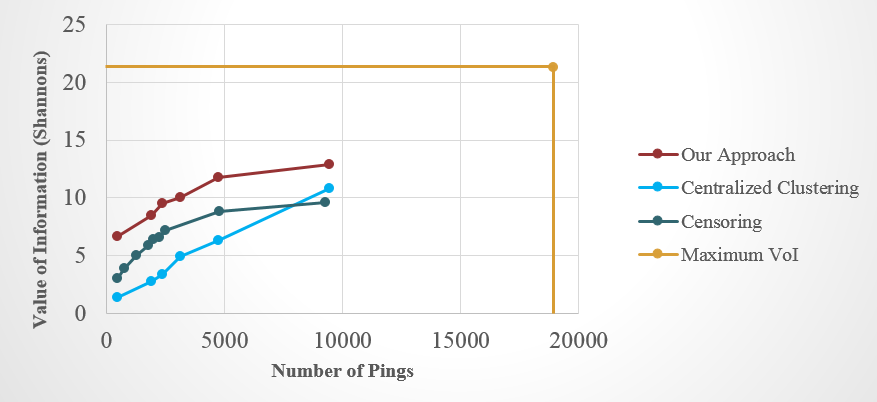
\includegraphics[height = 80mm, width = 120mm, scale = 2]{figs/Result1}
\caption{Information gathered vs Number of pings \textemdash TelosB sensor data}
\label{telosb}
\end{center}
\end{figure}
%INSERT FIGURE 4.1
\begin{figure}
\begin{center}
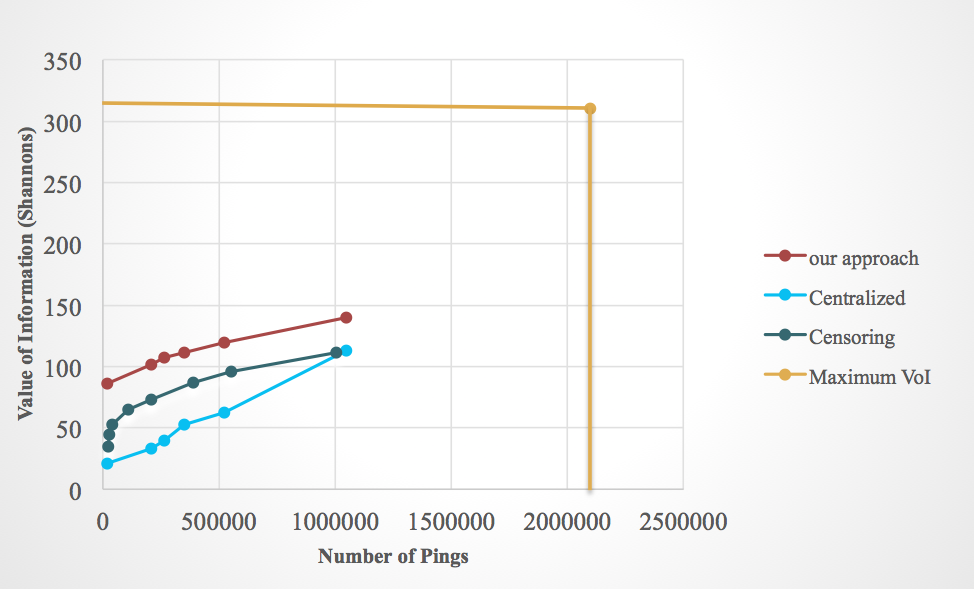
\includegraphics[height = 80mm, width = 120mm, scale = 2]{figs/Result2}
\caption{Information gathered vs Number of pings \textemdash Intel Research Lab data}
\label{intel}
\end{center}
\end{figure}
%INSERT FIGURE 4.2
In the first experiment, we considered data from the TelsoB sensors
\cite{suthaharan2010labelled}, and as stated in the algorithm above,
we calculate the entropies for each measurement of this data using
entropy equation. Next, we calculate the TM\textsubscript {VoI}
available in the data set using Algorithm \ref{tmvoi}. This will help
us understand how each model will rank against the overall information
available in the network. Next, using Algorithm
\ref{sensor-selection}, we run the simulator with this data set by
varying the number of pings. The variation in pings gives us a measure
of how each model is performing at different rates of sampling.
Obviously, the more a network is sampled, the more information can be
collected, but when we are dealing with networks that are on an energy
budget, we cannot afford sensors that perform excessive transmissions,
as it would deplete the network much faster than expected.

Figure \ref{telosb} illustrates the performance of all the models in
consideration, in terms of the amount of information gathered at
different ping rates for data gathered by the TelosB sensors in
\cite{suthaharan2010labelled}. We can clearly see that our model
outperforms both the models at each variation of the ping rate. In our
second experiment, we considered the Intel Lab data
\cite{BodikGuestrinEtAl2004}, and followed the same procedure outlined
in Section \ref{methodology}: initially determining the theoretical
maximum VoI available in a system and later choosing the informative
sensors using algorithm \ref{sensor-selection}. From Figure
\ref{intel}, we again notice our model gathering more information at
every variation in the ping rate, compared to the other two models.

Now, let us take a look at the reasons behind the performance
variation and why our model would be an ideal implementation in order
to increase the amount of information being gathered. Although both
the models chosen for comparison intend to increase the per-ping
information gathered while reducing the number of transmissions, they
were developed with the intent of discarding the information gathered
by sensors in most cases. Considering
\cite{muruganathan2005centralized}, the cluster head (CH), after
gathering information from each sensor within the cluster, performs
data aggregation and discards most of the data, sending only part of
the information gathered.  Moreover, this approach consumes extra
transmissions at every time step, as each CH again needs to transmit
information to the sink. \cite{rago1996censoring} on the other hand,
uses Likelihood Ratio (LR, defined as the dual of the ratio of the probability of
false positives and false negatives.) %%%%% IMPORTANT: DEFINE LR BEFORE USING ACRONYM %%%%% 
to transmit information to the sink. Sensors found to have LR with enough
information report information to the sink node.  Our experiments
showed that there were many instances where LR was found to be low which
resulted in excessive transmissions. Also, implementing such a decentralized 
model means that sensors will have to deal with the problems reviewed in 
Section \ref{intro}.  We also feel that if the computed LR were quantized, 
the information gathered would be higher for this approach than computed. The 
performance of our model is entirely dependent on the probability model proposed 
in Section \ref{methodology}. The algorithm, at every time step, is able to choose 
particularly informative sensors, thereby gathering more information on comparison
to other models.

The following implication can also be made from the graphs. As we
know, more information can be gathered from a network if it is sampled
more often, meaning that one would expect to see an asymptotic graph
with the previous statement taken into consideration. This can be seen
in all of the models in both of the experiments.

\begin{figure}
\begin{center}
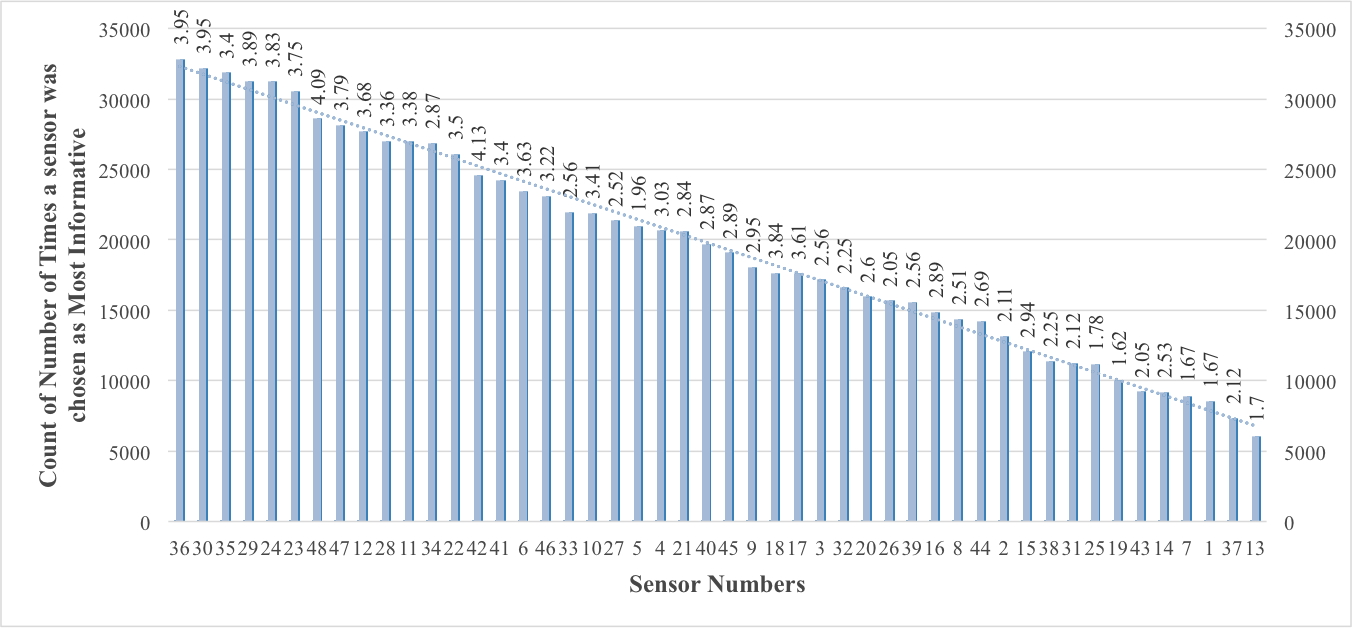
\includegraphics[height = 100mm, width = 150mm, scale = 1]{figs/Result3}
\caption{Ranking of the sensors according to the number of times chosen as Most-Informative}
\label{most-informative}
\end{center}
\end{figure}
% INSERT FIGURE 4.3
In our third experiment, we considered the Intel data set, and queried
all of the 48 sensors considered by slowing the ping rate down to 1/2
of the original.  This ping rate was chosen as a good illustration of
the network performance in terms of the amount of information
gathered. A graph was then plotted against individual sensors and the
number of times each sensor was chosen at different time steps. Figure
\ref{most-informative} shows the ranking of the sensors (from left to
right) in terms of the number of times each sensor was selected for
querying. This plot shows the consistency of the model in choosing the
sensors at each instant. Figure \ref{most-informative} is further
proof to the results above that our model correctly queries sensors at
an appropriate rate, given the amount of information predicted for
each sensor. We can also observe that the sensors gathered a
proportional amount of information with respect to the times they were
sampled. For example, sensor 36, which was chosen highest times
(approx. 32000) gathered close to 4 Shannons of information, while
sensor 26 gathered 2.05 Shannons over approximately 17000 samples.
The trend line in the graph shows the average number of queries sent
to each sensor.
%INSERT FIGURE 4.4
\begin{figure}
\begin{center}
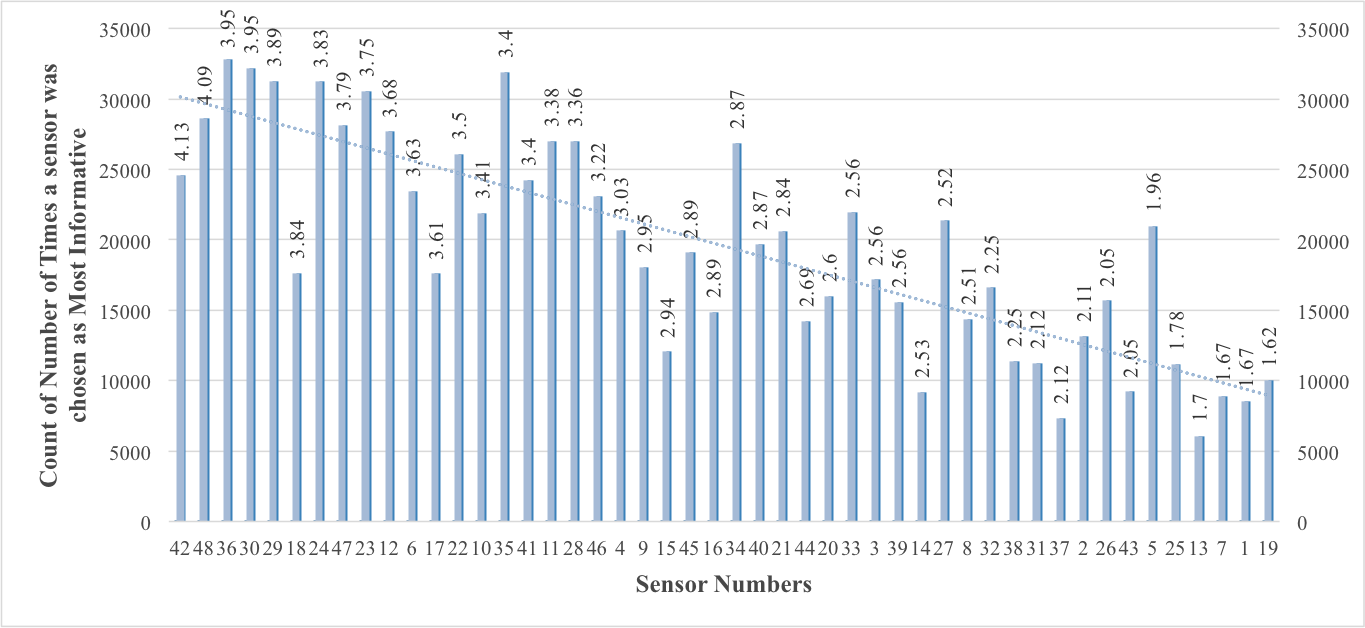
\includegraphics[height = 100mm, width = 150mm, scale = 1]{figs/Result4}
\caption{Ranking of the sensors according to amount of Information Gathered}
\label{info-gathered}
\end{center}
\end{figure}

In our final experiment, considering the same assumptions as in our
previous experiment, we plot a graph against sensor number and the
times each sensor was chosen as most informative but, this time to show
the overall VoI gathered by them. Figure \ref{info-gathered} shows the ranking
of the sensors (from left to right) in terms of the amount of information gathered
by them during a run. Our model always randomly selects a sensor based on
the current VoI gathered, not on the theoretical maximum VoI (which is not
accessible to an on-line algorithm). If that were the case, we would
have seen a result similar to figure \ref{most-informative}. However,
as the VoI distribution changes constantly with every query at every
time step, we do not see a smooth slanting curve. For the same reason,
we can also observe that certain sensors have been queried less often,
although in the end they provided a greater amount of information, and
vice-versa. However, the trend line in the graph is proof that, sensor selection
is proportional to the number of times each sensor is being queried. It also
shows the average amount of information gathered by each sensor. From
these analyses, we can clearly see how our model outperforms other state-of-the-art models,
both in terms of information collection and energy efficiency.
\chapter{CONCLUSION}
In this paper, we started off by proposing a model that is best
suitable for WSNs that are going to be built on an energy budget. We
stated several reasons why a centralized architecture with a
high-energy central node would be beneficial in comparison to a
distributed architecture. Next, we proposed a novel entropy-based VoI
approach for a centralized network to determine the theoretical
maximum VoI present within a network. We also present a
probability-based sensor selection algorithm to consistently select
informative sensors, enabling the model to increase the amount of
information gathered from a network. Moreover, by varying the sampling
rate, we have shown that our model can extract a high amount of
information even at very low sampling rates.

The performance of our approach was compared to two state-of-the-art
techniques (clustering for a centralized WSN and distributed
self-censoring) currently being employed to increase both the amount
of information being gathered and the energy efficiency. We developed
a simulator emulating all three models, and results clearly show that
our approach gathers more information per ping, implying that it is
more energy-efficient than the comparison models. Hence, we conclude
that our model provides an energy-efficient approach for increasing
the information gathered from a centralized network.
%
\nocite{*} % Use to exclude specific citations from *.bib file
\bibliography{References}
\bibliographystyle{ieeetr}%{alpha}%{ieeetr}%%
%\appendix
%\input{appendix}
\newpage
 \begin{vita}{Sushyanth Pamulaparthy}{Master of Science}{Computer Science} %Creates vita
 \vitaitem{Personal Data:} Born in Hyderabad, Telangana, India on February 6, 1992
 \vitaitem{Education:} \\ Received the B.Tech degree from Jawaharlal Nehru Technological University Hyderabad, Telanagana, India 2013\\
Completed the requirements for the degree of Master of Science with a major in Computer Science at Oklahoma State University in July, 2015. 
%\vitaitem{Experience:} \\ Tons of experience doing very cool things!
  \end{vita}

%       \pagestyle{empty}

\end{document}
